\subsection{
  Replies to comments received from Phillip Litchfield - Feb 14, 2013 }

\begin{enumerate}

%........................................................................................................
\vspace{5 mm}
\item
{\em
  ``L178:
"S[m;r';f]"  i think that should be S[m;t;r';f]?
}\\
\\
Correct, fixed in v4.

%........................................................................................................
\vspace{5 mm}
\item
{\em
	``L359f \& F12:
Doesn't the effect of s[12] s[13] dm2[12] depend on the value of s[23] not just s22theta[23]?  Are both octants considered in F12?  Is that the reason for the sign flip at $\sim$0.0025eV$^2$?
}\\
\\
The effect of the non-23 sector parameters does depend on the octant,
but the effect is small \& we assume the  $\theta_{23} < 45^\circ$
octant throughout.
%PLEASE CONFIRM MY LOGIC:
%NICKS CODE
%double s23 = sqrt(0.5 * (1 - sqrt(1 - sinsq2theta23)));
%I CHECK THIS
%for(double i = 0; i <= 1; i+=0.01) cout << asin(sqrt(0.5 * (1 - sqrt(1 - i))))*180/TMath::Pi() << endl;
%ANSWER IS 0-45 degrees
The reason for the sign flip in Fig 12. is a complicated interplay of
4 parameters, and so no simple statement like 'above the line,
$\sin^22\theta_{13}$ is small; below the line $\sin^22\theta_{13}$ is
large' can be made.

%........................................................................................................
\vspace{5 mm}
\item
{\em
	``L440f:
Later on it's said that the parameters are allowed to go out to 5sigma. What happens outside the 3sigma range? (It seems that this is not important in practice)
}\\
\\
The response functions are made using TSpline3's; they are perfectly
valid to be evaluated outside their range. An example is shown in
Fig. \ref{fig:spline_extrapolation}.
In practice, systematics rarely leave the $\pm 3 \sigma$ range (see
Fig. 398).

\begin{figure*}[htb]
%\begin{minipage}[t]{0.48\linewidth}
\center
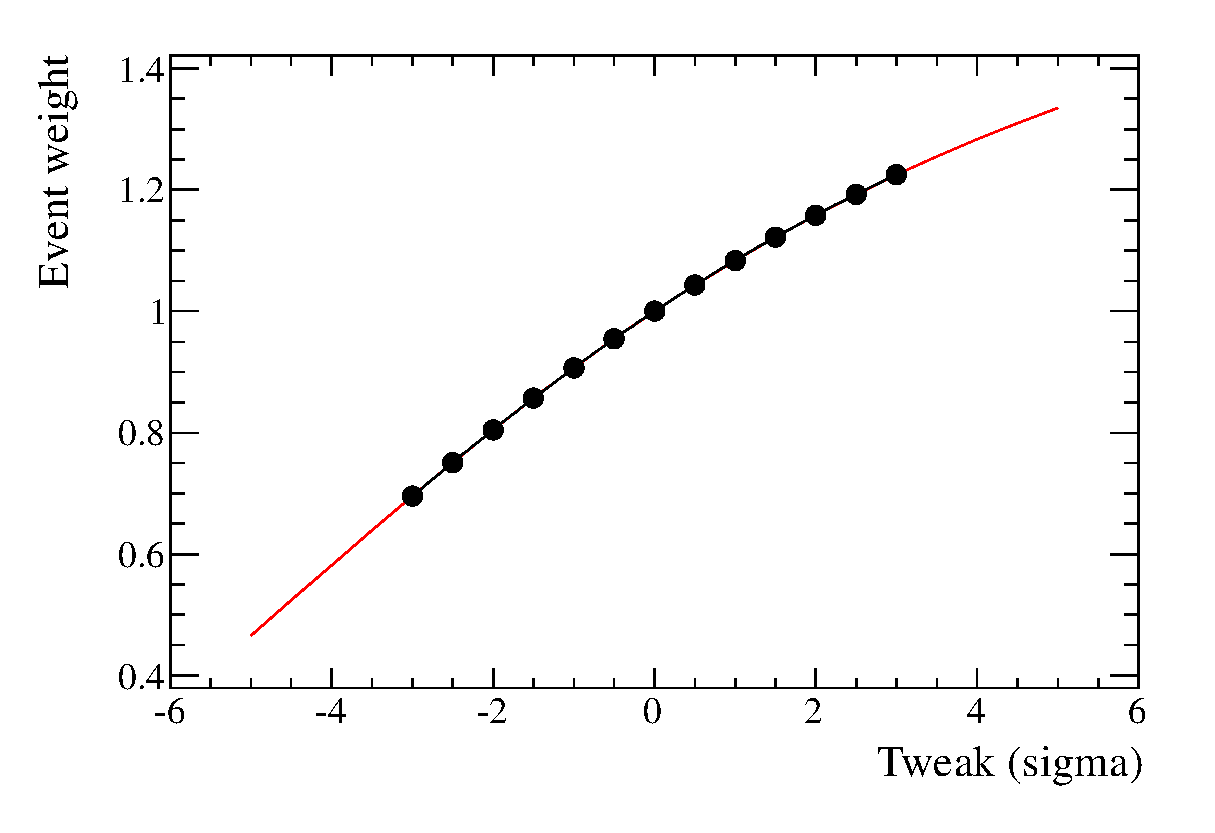
\includegraphics[width=20pc]{./images/spline_extrapolation}
\caption {
  Example of a cross-section spline; this shows the event weights obtained by tweaking $M_{A}^{RES}$
  for $\nu_{\mu}$-1$\pi$ events in the bin with reconstructed energy 0.4-0.45 GeV and 
  true energy 0.7-1.0 GeV.
  A graph showing the extrapolation of the spline beyond $\pm3\sigma$
  is shown.
}
\label{fig:spline_extrapolation}
%\end{minipage}
\end{figure*}

%........................................................................................................
\vspace{5 mm}
\item
{\em
	``L497f:
Is the spectral function penalised in the same way as the other errors? (i.e. full SF model +1 sigma gets on unit of chi2?)  Or is it free to move in the [0,1] range?  It wasn't clear and i could imagine arguments for either approach.
}\\
\\
The spectral function is penalised in the same way as the other errors.

%........................................................................................................
\vspace{5 mm}
\item
{\em
	``L717f:
I think this is answering a question was about to ask:  If you move the QE E$<$1.5 Gev parameter up by Nsigma, what happens to the QE E $>$1.5 parameters?
But i wan't quite sure i understood what this paragraph meant, mathematically.  [If we ignore the others parameters] would say, the f(banff)$_{19}$ be bundled as (correlation coeff) * f(banff)$_{18}$? And in general just adjust the non-fit parameters to the minimum of the N-8 hyper-elipse defined by the fit parameters?
}\\
\\
Please see the reply to Neil's comment \#7.

%........................................................................................................
\vspace{5 mm}
\item
{\em
	``Fig24-27:
You might guess that I approve of the star plots. ;)  But the thing i take from these is that the susceptibility of our analysis to the nuisance parameters is incredibly asymmetric (which means non-Gaussian at least and is worrying to deal with, as it opens up so many "what if?" scenarios).  I've never seen 'stars' that look this bad.  Are the plots correct?
}\\
\\

The plots have been found to be incorrect. The -1$\sigma$ fit was done
for a toy experiment created at the +1$\sigma$ best fit point, rather
than the test point. This caused the asymmetric errors. The plots have
been updated in v5 of the note.

%%%%%% ORIGINAL ANSWER %%%%
% The plots are correct.
% Fig. \ref{fig:different_dmsq} shows the
% effect on the 1-ring $\mu$-like spectrum, when changing $\Delta m^2_{32}$
% for fixed $\sin^22\theta_{23}$.
% It can be seen that the response in each bin is not symmetric.

% \begin{figure*}[htb]
% %\begin{minipage}[t]{0.48\linewidth}
% \center
% 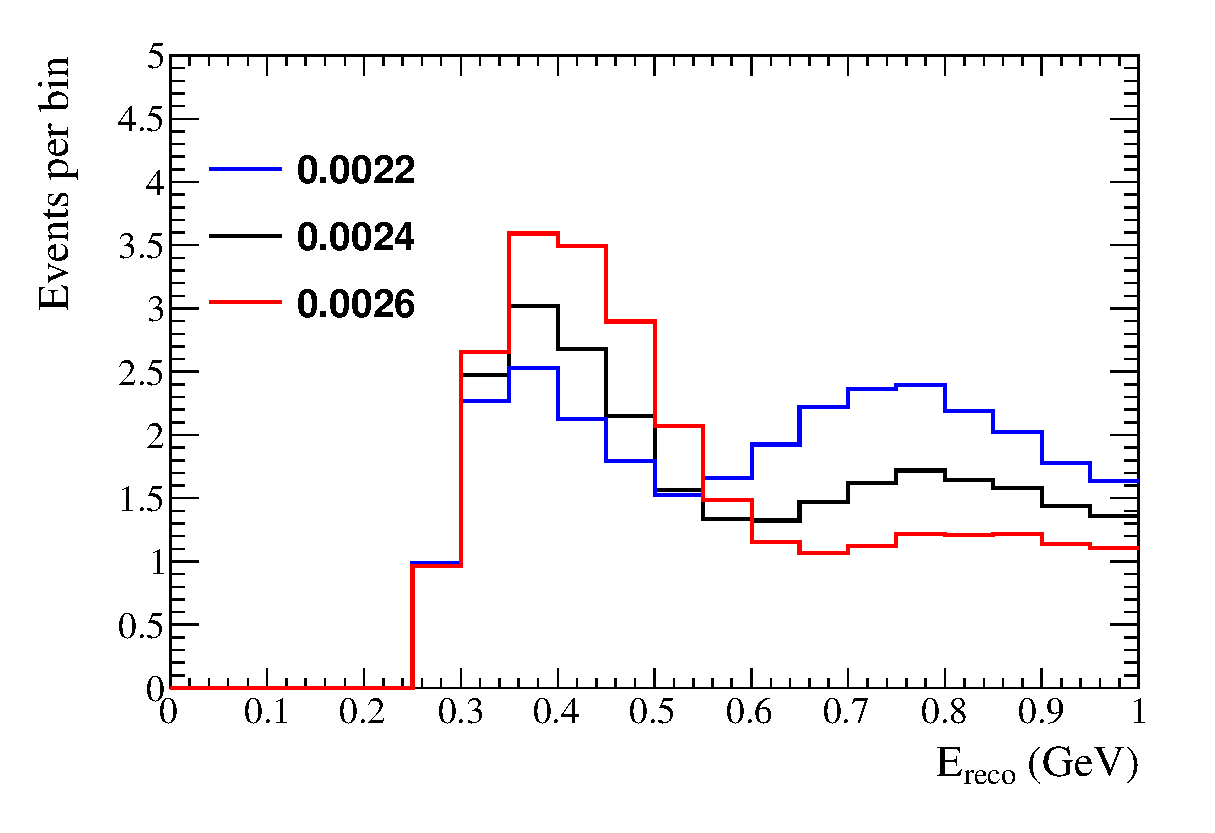
\includegraphics[width=20pc]{./images/different_dmsq}
% \caption {
%   1-ring $\mu$-like spectra for different values of $\Delta m^2_{32}$.
%   $\sin^22\theta_{23} = 1.0$, and the 2012 PDG values are
%   used for the non-23 sector oscillation parameters, with $\delta_{CP} = 0$.
% }
% \label{fig:different_dmsq}
% %\end{minipage}
% % \hspace{0.06\linewidth}
% % \begin{minipage}[t]{0.48\linewidth}
% % \center
% % 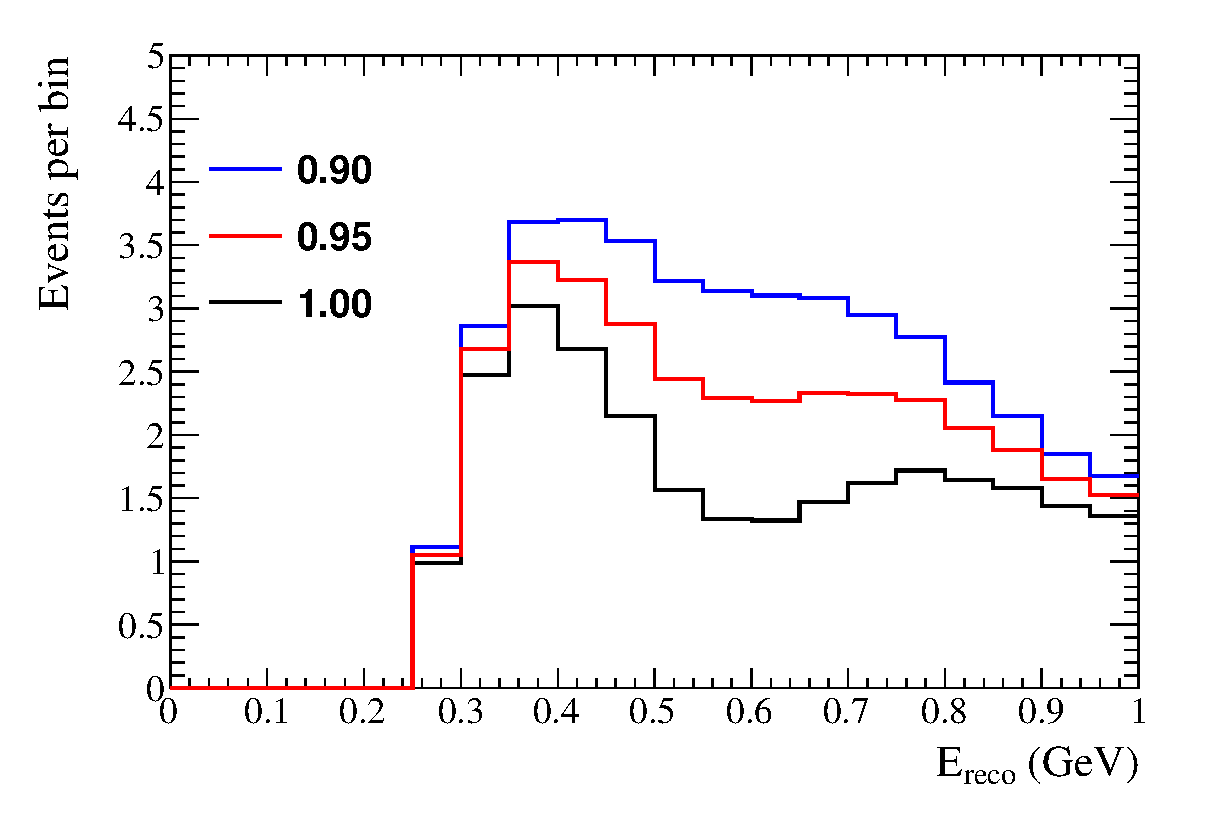
\includegraphics[width=20pc]{./images/different_mixing}
% % \caption {  
% %   1-ring $\mu$-like spectra for different values of
% %   $\sin^22\theta_{23}$. $\Delta m^2_{32} = 0.0024$, and the 2012 PDG values are
% %   used for the non-23 sector oscillation parameters, with $\delta_{CP} = 0$.
% % }
% % \label{fig:different_mixing}
% % \end{minipage}
% \end{figure*}



%........................................................................................................
\vspace{5 mm}
\item
{\em
	``L742:
I would disagree that the constant delta chi2 method can be characterised as "fully frequentist".  Yes it is in the case where the likelihood is Gaussian and the same width everywhere etc etc. But that's pretty much just saying it's fully frequentist 'in the special case where the frequentist analysis happens to coincide with the constant chi2 method'.  Constant delta chi2 is also fully Baysean under a not-dissimilar set of conditions.   Moreover we know the boundary is important, and that away from the boundary the likelihood is not elliptical.  So we knew ahead of time that the Gaussian approximation would not be valid here.
}\\
\\
We already say this: ``It is a fully frequentist treatment using the Gaussian approximation.``

%........................................................................................................
\vspace{5 mm}
\item
{\em
	``L749:
I don't think it's right to say that classical methods will undercover or overcover. 
The classical construction of which the F\&C method is just a particular variant does provide correct coverage 
(as much as quantisation allows) essentially by definition. The coverage problems discussed in the F\&C paper are only 
due to the hypothetical analyser not following the classical prescription correctly.   The empty region bit is right though.
}\\
\\
The statement made in the paper is correct. 
In that context, `classical construction' refers to the constant-$\Delta \chi^2$ method, not to the Neyman construction.
The constant-$\Delta \chi^2$ method, as described in Sec. 4.5.1, does not use the freedom which is inherent in the Neyman construction.
The method clearly does not have correct coverage as it can be seen in Figs. 29-30.
We agree with your statement that, in the F\&C paper, the coverage problems discussed are due to flip-flopping.
But, even if the hypothetical analyser does not flip-flop, the constant-$\Delta \chi^2$ method can 
underover and overcover.

%........................................................................................................
\vspace{5 mm}
\item
{\em
	``F28,29,30:

Is there something going on in the left corners of F28, and the equivalent slices? It looks like there some fairly large regions that are just set to 2.30 or 4.61. Is that correct?  If these plots are for external consumption i think it would it be better to make these regions blank.
}\\
\\
Correct; using the result of the constant-$\Delta \chi^2$ method we reduced the number of points we made the FC surface for (purely for computational time reasons).
We will update the plots to be white for points where we have not
performed FC in v5 of the note.

%........................................................................................................
\vspace{5 mm}
\item
{\em
	``F40-47:

It would be nice to have the 0-1 region take up more of the ratio plots. Since they are ratios,  a log axis might work?
}\\
\\
We feel that the plots are ok. Figs. 39-44 show the result with the
fit binning (73 bins) and so suffer from problems with a high
statistical error - this makes it both hard to plot \& hard to make
conclusions.
That is the purpose of Figs. 45 \& 47 (with 20 coarse bins). We will update these 2 plots
with a taller bottom TPad in v5 of the note.

 
%........................................................................................................
\vspace{5 mm}
\item
{\em
	``L835:
For clarity, i'd like to know what you meant by marginalise here.  Is the other oscillation parameter marginalised by MC integration, as with the systematics, or are you summing over the 2D distribution?
Or something else?
}\\
\\
We use the profile likelihood method. Taking the example of Fig 54.,
for a given $\Delta m^2_{32}$, we scan all bins in $\sin^2 2\theta_{23}$ and find the minimum value of the $\Delta \chi^2$ - this minimum is the value of the 
marginalised $\Delta \chi^2$ at the given point.


%........................................................................................................
\vspace{5 mm}
\item
{\em
	``L902:
Again, disagree that the constant delta chi2 contours can be said to have correct coverage, as we know the likelihood function will not obey the necessary conditions over the interesting range of parameter space. 
At the most basic level, if the best fit is up against the boundary, then you are not starting your delta chi2 from the tip of Gaussian peak.  But even if that were fixed, i'm dubious about whether the required Gaussian conditions would apply.
}\\
\\
The list we gave is the requirements from the muon-neutrino contour
committee, and not what the constant-$\Delta \chi^2$ method achieves.
We have clarified the language in v4 of the note.


%........................................................................................................
\vspace{5 mm}
\item
{\em
	``L922:
I agree that the 2+8 analysis is better presentationally. (i) Systematic errors area dark art, in many cases we are just trying to parameterise ignorance. Letting the fit flail round through a large number of parameters doesn't do anything against the problem that something might just be flat wrong, and may actually increase it. (ii) I'm not particularly inclined to believe the fitters mapped that space fully either: as a grid, 2 points per parameter would still be 10$^{14}$ evaluations. So it seems more defensible to reduce the dimensionality ourselves rather than let MINUIT do it implicitly. (iii) And from a presentational standpoint: Given that we may want to increase the complexity of our data sets over time, and that this generally makes the fitters slower, we run the risk of a climbdown in future analyses if we trumpet how many parameters we are fitting this time round.
}\\
\\
We agree (which is why we pursued the '2+8' result), but also see the response to Scott's comment \#3.

\end{enumerate}
